\documentclass[tikz,border=10pt]{standalone}
\usepackage{tikz}
\usetikzlibrary{arrows.meta,positioning,fit,backgrounds}

% ---------- Styles ----------
\tikzset{
  data/.style={
    draw, rounded corners, fill=gray!10,
    text width=34mm, minimum height=10mm,
    align=center
  },
  proc/.style={
    draw, rounded corners, fill=blue!6,
    text width=54mm, minimum height=12mm,
    align=center
  },
  smallproc/.style={
    draw, rounded corners, fill=blue!6,
    text width=58mm, minimum height=10mm,
    align=center
  },
  note/.style={
    draw, rounded corners, fill=yellow!15,
    text width=68mm, align=left
  },
  arrow/.style={-{Latex[length=3mm]}, line width=0.8pt, shorten >=3pt, shorten <=3pt},
  group/.style={draw, dashed, rounded corners, inner sep=6pt}
}

\begin{document}
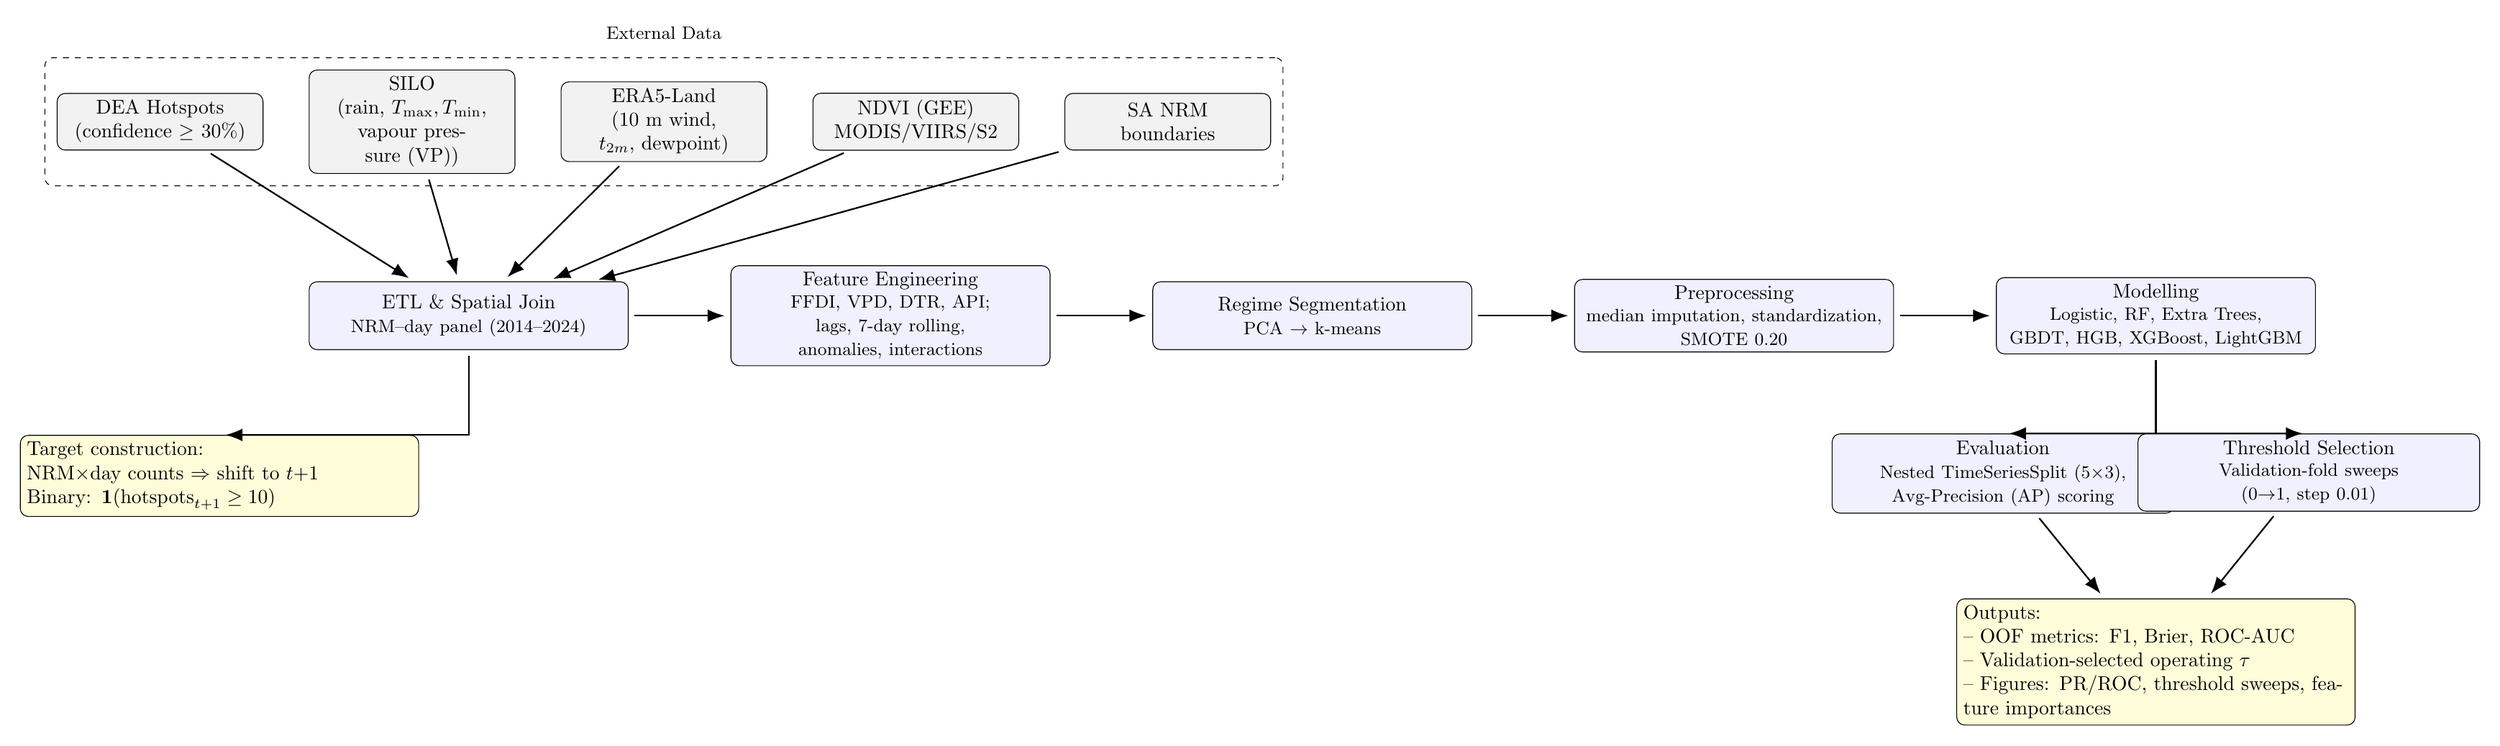
\begin{tikzpicture}[node distance=13mm]

% ---------- External data ----------
\node[data] (dea)  {DEA Hotspots\\(confidence $\ge 30\%$)};
\node[data, right=8mm of dea] (silo) {SILO\\(rain, $T_{\max},T_{\min}$,\\ vapour pressure (VP))};
\node[data, right=8mm of silo] (era5) {ERA5-Land\\(10 m wind, $t_{2m}$, dewpoint)};
\node[data, right=8mm of era5] (ndvi) {NDVI (GEE)\\MODIS/VIIRS/S2};
\node[data, right=8mm of ndvi] (nrm)  {SA NRM\\boundaries};
\node[group, fit=(dea)(silo)(era5)(ndvi)(nrm),
      label={[yshift=2mm]above:\small External Data}] (ext) {};

% ---------- Core pipeline ----------
\node[proc, below=19mm of silo, xshift=10mm] (etl)
  {ETL \& Spatial Join\\\small NRM--day panel (2014--2024)};

\draw[arrow] (dea)  -- (etl);
\draw[arrow] (silo) -- (etl);
\draw[arrow] (era5) -- (etl);
\draw[arrow] (ndvi) -- (etl);
\draw[arrow] (nrm)  -- (etl);

\node[proc, right=18mm of etl] (feat)
  {Feature Engineering\\\small FFDI, VPD, DTR, API;\\ lags, 7-day rolling, anomalies, interactions};
\draw[arrow] (etl) -- (feat);

\node[proc, right=18mm of feat] (reg)
  {Regime Segmentation\\\small PCA $\rightarrow$ k-means};
\draw[arrow] (feat) -- (reg);

% --- NEW: preprocessing box (as implemented in your pipeline) ---
\node[proc, right=18mm of reg] (pre)
  {Preprocessing\\\small median imputation, standardization,\\ SMOTE 0.20};
\draw[arrow] (reg) -- (pre);

\node[proc, right=18mm of pre] (model)
  {Modelling\\\small Logistic, RF, Extra Trees,\\ GBDT, HGB, XGBoost, LightGBM};
\draw[arrow] (pre) -- (model);

% ---------- Evaluation & thresholds (parallel under model) ----------
\node[smallproc, below=14mm of model, xshift=-27mm] (eval)
  {Evaluation\\\small Nested TimeSeriesSplit (5$\times$3), Avg-Precision (AP) scoring};
\node[smallproc, below=14mm of model, xshift=27mm]  (cal)
  {Threshold Selection\\\small Validation-fold sweeps\\\small (0$\rightarrow$1, step 0.01)};

\draw[arrow] (model.south) |- (eval.north);
\draw[arrow] (model.south) |- (cal.north);

% ---------- Outputs ----------
\node[note, below=15mm of eval, xshift=27mm] (out) {Outputs:\\
-- OOF metrics: F1, Brier, ROC-AUC\\
-- Validation-selected operating $\tau$\\
-- Figures: PR/ROC, threshold sweeps, feature importances};
\draw[arrow] (eval) -- (out);
\draw[arrow] (cal)  -- (out);

% ---------- Target construction ----------
\node[note, below=15mm of etl, xshift=-44mm] (target) {Target construction:\\
NRM$\times$day counts $\Rightarrow$ shift to $t{+}1$\\
Binary: $\mathbf{1}(\mathrm{hotspots}_{t+1}\ge10)$};
\draw[arrow] (etl.south) |- (target.north);

\end{tikzpicture}
\end{document}
